\documentclass[11pt]{article}
\usepackage[a4paper,margin=25mm]{geometry}
\usepackage{fontspec}
\setmainfont{TeX Gyre Pagella}
\setsansfont{TeX Gyre Heros}
\usepackage{microtype,booktabs,array,graphicx,enumitem}
\usepackage[numbers,sort&compress]{natbib}
\usepackage[colorlinks=true,linkcolor=black,citecolor=black,urlcolor=blue]{hyperref}
\usepackage{tikz}
\usetikzlibrary{arrows.meta,positioning}
\setlength{\emergencystretch}{3em}
\setlength{\parskip}{4pt}
\setlength{\parindent}{1em}
\title{GameSave2Minecraft: Agent-Guided Migration of Game Saves into Playable Minecraft Worlds}
\author{Alex Chengyu Li\\\small Independent Researcher\\\small\href{https://orcid.org/0009-0008-4516-8946}{ORCID: 0009-0008-4516-8946}}
\date{17 October 2026}
\begin{document}
\maketitle
\begin{abstract}
Player-built worlds combine spatial arrangements, visual resources and states that
make objects usable. Migrating such a world into Minecraft requires recovering
these relationships and assigning target interactions to its objects.
GameSave2Minecraft organizes this work as an agent-guided method: a source adapter
recovers a saved world using local game artifacts and reverse-engineering
evidence; a shared scene contract separates definitions, instances and state;
interaction rules give migrated objects Minecraft placement, collision, use and
persistence; and acceptance checks bind the resulting world to source coverage
and measured runtime behavior. New games enter through adapter and rule
development. A reference implementation includes an original procedural source
format, deterministic scene compilation, a reusable Minecraft runtime and
reusable instructions for coding agents. A V Rising case reconstructs four
saved castles containing 12,057 visible objects and 182 terrain patches, and
retains 1,044 inventory entries with their original slots and quantities.
Doors, seats, beds, lights and plants receive explicit target behaviors. In a
single paired RTX 3090 session with one twenty-second window per build and a
30-frame-per-second cap, interior median render
work falls from 162.64 to 13.81 milliseconds while observed frame rate rises from
4.61 to 29.19. The case demonstrates how source recovery, interaction mapping and
world-scale rendering can form one inspectable migration process.
\end{abstract}

\section{Introduction}

A player-built castle is a collection of commitments. A staircase connects
floors, a door controls a passage, a chair offers a place to sit, and a container
holds the results of earlier play. The save records some of these commitments;
the game client supplies models, materials and executable rules that make the
records meaningful. Moving the castle into another game therefore involves
reconstructing an assembled, usable place from several kinds of evidence.

Minecraft is a useful destination because its worlds support persistent editing,
multiplayer use and an extensive mod interface. A migrated castle can become a
place that its owner revisits, rearranges and incorporates into further play.
The desired result has both spatial and behavioral obligations. A recognizable
door needs a selected hinge and a collision update when opened. A source coffin
can receive Minecraft sleeping behavior. A chair needs a seating position and
an occupancy rule. These decisions determine whether the migrated environment
functions as a world for players.

This paper develops GameSave2Minecraft as a general method for game-save migration.
The inputs are a source save, a matching locally available game installation and
its required content, together with a selected Minecraft target. A coding agent
investigates the source, authors or extends a source adapter, and connects its
output to a reusable world contract and target runtime. The adapter is developed
as part of the migration, allowing the workflow to address source games for
which no converter has been prepared. The common work comprises interaction
rules, deterministic world construction, state persistence, performance
engineering and acceptance.

The contribution is an executable organization of that process. First, the world
contract keeps object definitions, saved instances, state and recovery evidence
separately inspectable. Second, capability rules connect recovered objects to
Minecraft interactions with observable persistence and failure conditions.
Third, the runtime and acceptance procedure address the cost of retaining a
large population of individually usable objects. A source-bound V Rising case
provides concrete recovery, interaction and performance observations. An original
procedural source format supports public inspection and repeatable tests without
redistributing a commercial game's art or a player's save.

\section{Related work and design position}

Cross-game conversion has concrete precedents. MineCity 2000 reads SimCity city
files and constructs Minecraft terrain and buildings through a source-specific
reader and a library of target buildings.\cite{minecity} This establishes a useful
save-driven pattern: saved placement data selects reusable target definitions.
KindredSchematics provides castle export and import within V Rising, including
territory and castle-heart relationships.\cite{kindred} Its source-game building
relationships informed the investigation of the case in this paper.

Agent tooling expands the practical routes available for such work. REA exposes
artifact inspection and reverse-engineering capabilities to coding agents across
managed, native and packaged targets.\cite{rea} Universal Modder supplies agent
skills for game investigation, asset pipelines, cross-game content ports and
other forms of game combination.\cite{universal} These projects are relevant
substrates and close comparators. GameSave2Minecraft develops the specific
end-to-end contract of a saved source world becoming an editable, persistent
Minecraft world, with object coverage and capability acceptance carried through
the conversion.

Scene interchange formats provide established representations for geometry and
assembly. Khronos describes glTF as a format for delivering scenes, meshes,
materials and animation.\cite{gltfrelease} A migration also needs the meaning of a
saved object: its inventory, selected appearance, interaction state and target
use policy. The shared contract consequently includes source state and
capabilities alongside visual references. Its purpose is to connect a source
adapter to a target runtime while making that additional information explicit.

Game preservation also includes players' experiences of familiar places. Smith
Nicholls and Cook use go-along interviews in Wurm Online to study a persistent,
player-directed world and its culture.\cite{wurm} Their work highlights the
interpretive value of inhabiting and explaining a place. Here the engineering
question is how an existing saved place can acquire a further playable
representation whose transformations can be inspected.

\section{The migration method}

\subsection{Recovering a source world}

The investigation begins by identifying the save, client version, enabled
content and resource carriers. A save may refer to prefabs, items or variants
whose geometry and behavior reside elsewhere. Recovery follows those
dependencies from saved instances to definitions, renderer parts, materials and
state. The source adapter records the identities of its inputs and tools, the
fields it recovered and any unresolved relationships. Each in-scope object must
receive a reconciled outcome.

REA can help establish binary and package structure, relevant serialization code
and runtime bindings. The agent chooses additional asset tooling according to
the source engine. For a managed game, direct assembly inspection may expose the
needed types. For a game using Unity's IL2CPP backend, which compiles managed
code into native code, matching native and metadata artifacts can
support interop generation and focused layout recovery. A game's own runtime
can serve as a serialization oracle: it loads an isolated save and exports the
resolved entities through a bounded one-shot plugin. The choice depends on the
available evidence and the cost of interpreting a format directly.

The adapter interface separates probing, scene export and source verification.
Probing reports format, version and artifact identity. Export resolves object
definitions and saved instances into the shared contract. Verification compares
the export with independent saved data, an authoritative source API or a source
runtime readback. Structural validation then checks the normalized representation.
This separation makes a successful file parse distinguishable from a recovered
world that agrees with the source.

Composite objects require particular attention. An object may include several
meshes, selected renderer conditions, child transforms and material slots. A
saved plant may choose among several growth-stage appearances. A wall may carry
a selected surface treatment. Material tint alpha, texture cutout alpha and
shader blend mode also have distinct effects. The adapter resolves these
relationships before target resource generation, so that a component's identity
continues to describe the assembled object the player placed.

\subsection{A shared scene and capability contract}

The scene contract contains reusable asset definitions and independently
identified instances. An asset describes its visual references, bounds,
collision and selection geometry, and interaction parameters. An instance
describes its definition reference, transform, optional parent, saved state and
source binding. Coordinates are normalized to metres, Y up and a declared
handedness. Quaternion, scale and hierarchy checks reject non-finite values,
missing parents and cycles. Full affine matrices remain available when the
hierarchy is flattened. A target-specific bake resolves transforms that its
native object representation cannot directly express.

The coverage record reconciles expected source instances with migrated records
and explicit exclusions. Exclusions carry an identity and a reason; unresolved
references remain actionable records. An invisible source bookkeeping entity
can be documented separately from a visible furnishing. A character excluded
from a building migration has a different reason from a furnishing whose model
failed to decode. This accounting preserves the meaning of a completeness claim.
An extracted-asset ledger likewise assigns every model and texture an identity
and either mapped target resources or a reasoned exclusion, and is checked
against the extractor's inventory before acceptance.

State is kept independently of geometry. Inventory records retain source item
identity, amount and slot, with display names stored as descriptive fields. A quantity that exceeds a Minecraft stack limit can be represented by a
source-resource lot carrying the original amount. Unknown state can remain
attached to its source binding while a new capability rule is developed. The
target policy states which fields drive gameplay and which remain retained
source information.

Figure~\ref{fig:pipeline} shows the architecture. Source-specific work is concentrated
in the adapter and in any new capability rules. The scene contract, target
construction, existing rules and acceptance procedure are reused. New engine
families can therefore enter through the same development process, with their
recovered data checked before it is treated as target-world content.

\begin{figure}[t]
\centering
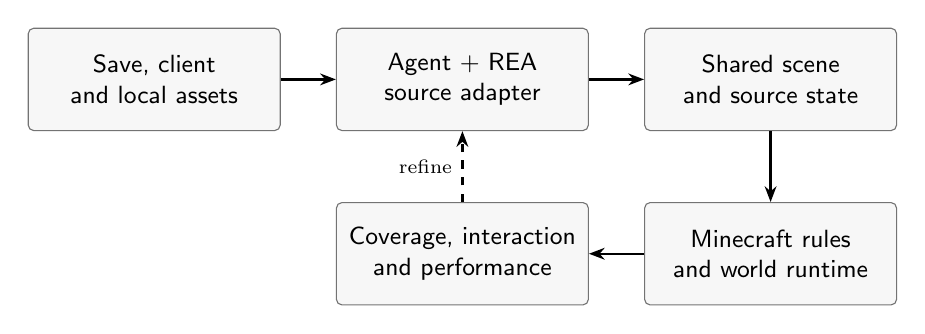
\begin{tikzpicture}[font=\small\sffamily,box/.style={draw=black!55,rounded corners=2pt,fill=black!3,align=center,minimum width=32mm,minimum height=13mm},arr/.style={-{Stealth[length=2mm]},thick}]
\node[box] (source) {Save, client\\and local assets};
\node[box,right=7mm of source] (adapter) {Agent + REA\\source adapter};
\node[box,right=7mm of adapter] (scene) {Shared scene\\and source state};
\node[box,below=9mm of scene] (target) {Minecraft rules\\and world runtime};
\node[box,left=7mm of target] (accept) {Coverage, interaction\\and performance};
\draw[arr] (source)--(adapter);
\draw[arr] (adapter)--(scene);
\draw[arr] (scene)--(target);
\draw[arr] (target)--(accept);
\draw[arr,dashed] (accept)--node[left,font=\scriptsize]{refine}(adapter);
\end{tikzpicture}

\caption{Agent-guided migration. Source artifacts supply recoverable definitions
and state; the shared contract connects them to target capabilities and world
construction. Acceptance compares the source, normalized scene and running
Minecraft result.}
\label{fig:pipeline}
\end{figure}

\subsection{Minecraftization through reusable interaction rules}

Minecraftization assigns an object a place in the target world's spatial and
behavioral systems. The reference rules cover doors, seats, beds, containers,
lights, plants, workstations and static components. Table~\ref{tab:rules} summarizes
the resulting obligations. Each rule connects appearance, selection, collision,
server state, synchronization and persistence. The rule vocabulary can grow
when another source mechanic requires a new target implementation.

\begin{table}[t]
\centering\small
\begin{tabular}{p{.14\linewidth}p{.34\linewidth}p{.43\linewidth}}
\toprule
Capability & Mapping parameters & Observable target behavior\\
\midrule
Door & Hinge, rotation, open state & Open/close, swept clearance, collision update, saved state\\
Seat & Seat and exit positions, occupancy & Mount, reject double occupancy, dismount, cleanup on removal\\
Bed & Sleep position, occupancy, dimension policy & Native sleep rules, waking and synchronized position\\
Container & Capacity, slot and resource mapping & Valid menus, quantity retention, carrying contents, reload\\
Plant & Stage appearances, timing, yield & Visible harvest and growth, single harvest, retained timing\\
Light & Active state and emission policy & Appearance and light update, synchronization, reload\\
Workstation & Target recipe and storage policy & Declared operations, valid menus and retained contents\\
\bottomrule
\end{tabular}
\caption{Common interaction contracts. Parameters and source-state mappings are
supplied by the adapter or explicitly selected target policy.}
\label{tab:rules}
\end{table}

A source door is represented by an owner identity and geometry that can span
several Minecraft cells. Opening it tests the new occupied volume, updates its
state and collision, and synchronizes the change. A seat uses an interaction
position and an owned seating entity; removing the seat or leaving it must
clean up that entity. A source coffin can use the bed rule and Minecraft's sleep
APIs. Containers use native menus with a declared capacity and a mapping from
source slots. NeoForge's block-entity interface provides persistence and update
mechanisms for state associated with placed blocks.\cite{neoforge}

The mapping is a design decision at the level of an object's use. For example,
a target workstation may expose a Minecraft crafting interface and retain its
source storage. Simulating the source game's recipes, fuel and progression
requires further rules. Recording the selected target policy allows the owner
to decide what continuing to use that object should mean. Artistic policies,
including pixel textures or block-based remodelling, can be applied while
retaining the same identity and interaction contract.

\section{World construction and runtime cost}

The target world keeps definitions reusable and instances separately editable.
Each object has a stable owner identity. Collision and selection fragments refer
to that owner, including fragments that extend into neighbouring cells. Breaking
or moving the object carries its retained contents. Generation uses deterministic
instance identities, proceeds incrementally and records completed regions. A
retry can restore the same object without producing a second identity or
resetting an already completed inventory. Owned chunk-loading tickets are
released at completion and interruption.

A selected target dimension or explicitly admitted placement region protects
existing builds from an import's placement operations. Safe entry checks actual
support and player clearance. Floors, stairs and doorways are therefore tested
through traversal as well as through metadata. Source recovery and target
construction can choose different internal representations while retaining the
same object-level obligations.

The number of occupied Minecraft cells can substantially exceed the number of
visual objects. Sending every collision cell through a generic block-entity
renderer introduces work even when that cell owns no visible geometry. The
runtime instead indexes loaded visual owners and renders them through a world
stage. Their visual bounds cover the complete transformed object and support
current-frame frustum and range tests. Lifecycle updates remove stale entries
after network changes, chunk unload and world transitions.

Static geometry, authored transforms and draw preparation can be cached. Cache
entries must invalidate when a resource or relevant object state changes. Weak
geometry references allow the bounded source-mesh cache to evict data; a prepared
plan resolves all dependencies before submitting work and uses an atomic
fallback after eviction. Frame-owned geometry references are released after
submission. Growing plants and articulated doors retain live transformations.

The GPU path groups compatible work by material and instances repeated geometry.
The OpenGL indirect-draw API supports submitting multiple indexed draws from a
command buffer.\cite{opengl} The implementation uses that capability where
available and retains a compatible rendering path. Blend, cutout, fog, overlay
and emissive behavior are checked against the reference renderer, and modified
rendering state is restored. Optional-mod adaptations are version-specific:
their observations must establish that only redundant work is removed and that
ordinary world entities remain intact.

Resource packaging is another part of the runtime contract. The program JAR
contains code and compact metadata; model payloads remain ordinary bounded files
in the user's existing resource distribution. Texture archive size, decoded
texture size and simultaneous GPU residency are different measurements. Source
texture processing and a rendering optimization must be reported separately so
that a faster frame cannot be attributed to an unmeasured compression change.

\section{Implementation and case evaluation}

\subsection{Reference implementation and original fixture}

The reference implementation supplies a Python adapter protocol, scene validator,
hierarchical transform handling, capability contracts, a deterministic partitioned
plan compiler and a Minecraft emitter. The target runtime uses Minecraft Java
1.21.1 with NeoForge. Its common component code provides stateful placement,
interaction and rendering. The generic runtime is extracted from the author-owned
component and renderer code evaluated in the case, with a separate namespace and
original demonstration assets. The accompanying \texttt{GameSave2Minecraft-0.1.0.zip}
contains this implementation and a Skill: reusable instructions and reference
contracts loaded by a coding agent when developing a new source adapter.
Opaque surfaces use the cached GPU path; translucent emissive surfaces use
Minecraft's camera-sorted buffers to preserve the ordering of overlapping faces.
The portable package stores complete world matrices;
the initial target emitter requires a declared bake for shear, reflection or
interaction configurations outside its implemented policies. Such requirements
remain explicit tasks for the agent and adapter.

An original miniature source format separates a compressed save from its client
catalog and visual resources. Its generator authors every fixture mesh and
texture. The demo adapter recovers fifteen saved instances using eight asset
definitions and verifies their records against the source save. The fixture
contains each common interaction family and a source-resource lot of 100,000
units in slot 37 of a 54-slot container. This fixture makes the adapter and target
contracts inspectable without needing a commercial game installation.

Twenty-five pure tests cover source-oracle agreement, extracted-asset accounting, transform composition,
dependency and hierarchy failures, non-finite data, missing growth appearances,
inventory identity and quantity, safe resource paths, topology, deterministic
output and package readback. Their scenarios are in \texttt{tests/} in the
accompanying archive. A larger fixture requests groups of at most 128 instances;
its 513 instances exercise several full groups and a one-instance tail while
retaining every identity. These tests exercise data and
compilation contracts. Native interactions and visual behavior are measured in
their own runtime lanes.

\subsection{Recovering four V Rising castles}

The empirical migration uses a player's V Rising save and matching local client
and dedicated-server artifacts, version 1.1.13. The evaluated migration mod is
version 0.2.1; version 0.2.0 supplies the performance baseline. The requested scope is the four
saved castle territories, their gardens and placed objects. The source
installation and original save remain unchanged. A one-shot exporter in an
isolated source server waits for scene streaming, enumerates the territory
entities and records object identities, transforms, ownership, component names
and inventory relationships.

Client resources provide the renderer and material assemblies. Matching client
and server marketing versions have different binary layouts, so their interop
and data observations are tracked separately. The recovery resolves all 987
saved prefab types needed by the territory export before target plan assembly.
Composite objects retain child transforms and selected renderer conditions.
The resulting scope contains 12,057 visible source objects. Another 6,172
logical or invisible entities and 98 character entities receive explicit
exclusion classifications. The latter belong to the territory enumeration but
fall outside the selected building-and-objects scope.

Material recovery exposed a consequential foliage case. Some cutout materials
use a zero alpha value in their colour tint while their albedo texture supplies
the actual cutout mask. Multiplying the two indiscriminately makes the plant
invisible. The conversion distinguishes opaque, cutout and transparent policies
and checks the resulting visible alpha. A material audit covers 1,074 native
configurations, including 112 zero-tint-alpha cutout cases. This illustrates why
source appearance requires interpretation of material behavior alongside mesh
and texture extraction.

The target plans retain source coordinates at one metre per Minecraft block,
with a common translation into the target dimension. A measured surface-based
collision conversion uses 0.125-metre cells and excludes foliage, cloth and
effects from solid volume. Source terrain queries supply 182 terrain patches;
unknown samples remain visible failures. Together the objects and terrain
produce 12,239 visual owners and 604,571 collision fragments across 283,035
component cells. Source geometry and placement remain intact through the
performance comparison.

\begin{table}[t]
\centering
\begin{tabular}{lr}
\toprule
Case property & Count\\
\midrule
Saved castle territories & 4\\
Visible source objects & 12,057\\
Measured terrain patches & 182\\
Target visual owners & 12,239\\
Source doors checked open and closed & 242\\
Objects with source storage capacity & 289\\
Retained source inventory lots & 1,044\\
Component cells / collision fragments & 283,035 / 604,571\\
\bottomrule
\end{tabular}
\caption{Recovery and target coverage for the selected V Rising case. Counts
describe this saved scene and its declared building-and-objects scope.}
\label{tab:coverage}
\end{table}

\subsection{Interaction and persistence acceptance}

The target adapts doors, seats, beds, lights, plants, containers and workstations
through the common interaction families. Source storage retains original slots,
names, identities, quantities and serialized source data. Each source-resource
token represents one retained lot. Plant timing and target yields use declared
Minecraft policies; recovered mature and growing appearances remain distinct.

The case passes nineteen native GameTest scenarios (automated server-side
tests that execute the mod inside Minecraft), thirty-eight actual packaged-client
scenarios and four renderer scenarios in a real OpenGL 3.2 context. Their
inventory is in \texttt{docs/case-summary.json} in the accompanying archive.
The client checks all four layouts and all 242 source doors in both open and
closed states. It
exercises native sleeping, seating, menus, lighting, harvesting, regrowth and
walking. Traversal of imported stairs and rendered comparisons of mature and
growing plants supplement the object-state checks.

Rendering controls compare the GPU path with a reference path, including lit and
unlit emissive materials, changed camera poses and resource-cache rebuilding.
Lifecycle checks remove and re-add a root through network updates and verify its
render-index membership. Distance checks cover the strict 256-metre boundary.
The optional culling integration excludes only the migration runtime's redundant
cells from the block-entity list inspected for visibility. An ordinary chest
remains in that list under both supported collection implementations.

The deployed program is approximately 5.2 MB, with approximately 960 MB of client
resources stored separately in ordinary repository files smaller than 2 MB each.
This keeps the program small while retaining the user's repository-based update
workflow; exact sizes and hashes are supplied in the case summary. The server
and client use the same program bytes. Save/load readback reconciles the visual
objects and 1,044 inventory entries, and preserves the castle region and
import-progress data after startup and a normal save.

\section{Matched performance observations}

The performance comparison uses the installed NeoForge 21.1.219 pack and native
OpenGL 4.6 on an RTX 3090 with NVIDIA driver 616.56. Both runs use the same initial
world, resources and pack configurations, fixed cameras, 1280 by 800 resolution,
four available processors, a 20 GiB heap ceiling and a 30 FPS cap. Before each
scene is timed, all 6,937 visual owners of the largest castle must be loaded;
the optimized run verifies each expected owner identity in its render index.

Each scene contributes every frame in one twenty-second measurement window per
build, from a single paired session. Before/after frame counts are 90/593 for
the overview, 93/584 for the interior and 591/594 for the looking-away control.
Interior diagnostic recordings run in a separate window afterwards, because
attaching a profiler can perturb compilation and garbage collection. The
optimized build is measured before the baseline build, and unrelated host work
continues during measurement. The fixed order and continuing host load limit
causal attribution to individual optimizations and the generalization of the
timings. Table~\ref{tab:performance} reports this paired session.

\begin{table}[t]
\centering\small
\begin{tabular}{lrrrrrr}
\toprule
 & \multicolumn{2}{c}{Render p50 (ms)} & \multicolumn{2}{c}{Render p95 (ms)} & \multicolumn{2}{c}{Capped FPS}\\
Scene & Original & Optimized & Original & Optimized & Original & Optimized\\
\midrule
Overview & 153.68 & 17.40 & 406.38 & 21.79 & 4.45 & 29.64\\
Interior & 162.64 & 13.81 & 217.07 & 19.69 & 4.61 & 29.19\\
Looking away & 2.50 & 2.54 & 3.76 & 3.31 & 29.54 & 29.69\\
\bottomrule
\end{tabular}
\caption{Matched case observations. Render work excludes frame-limiter sleep;
observed capped FPS includes frame spacing and client tick work. The statistics
summarize one measurement window per scene and build.}
\label{tab:performance}
\end{table}

Interior median render work decreases by 91.5 percent in this comparison. The
optimized overview and interior approach the selected frame cap while the
looking-away control remains near its earlier cost. The optimization retains
all source meshes, textures and placements. Its changes concern visible-owner
dispatch, prepared transformations, material batching and redundant optional-mod
snapshot work. These observations establish the delivered configuration's
before-and-after behavior. They provide the starting point for repeated,
counterbalanced experiments and per-component ablation on further sources and
hardware.

The acceptance procedure combines performance budgets with fidelity controls.
For this deployment the interior render-work targets are 16.7 ms at the median
and 33.3 ms at p95, and the overview median target is 25 ms. Relative to a
33.3 ms capped frame period, these targets reserve time for other client work
and bound slow rendering frames. The overview and interior must each sustain
at least 27 observed FPS, selected as 90 percent of the 30 FPS cap.
Identity coverage, visual comparisons, dynamic-state checks and successful
process exit accompany those budgets. Capped frame observations describe the
measured configuration; higher frame-rate targets require their own experiments.

\section{Discussion}

The method's generality resides in how unfamiliar source formats enter the
pipeline. An agent investigates the supplied game, generates its source adapter,
and extends capability rules where necessary. A common world representation
makes the results comparable even when their serialization and asset carriers
differ. The original fixture demonstrates that boundary with a separate source
format. The commercial-game evaluation establishes a complete migration case.
Further engine and save-format cases can measure how much new work remains in
the adapter, which rules transfer directly and which target mechanics require
extensions.

Interaction rules also make the meaning of preservation negotiable. A bed rule
can retain an object's use as a sleeping place, while the owner may choose a new
target rule for its source-specific recovery mechanic. A container can retain a
source quantity even when the target item behaves as a descriptive lot. The
mapping should preserve enough source information to make those choices
revisable. Human decisions about identity, recognizable appearance and intended
use remain part of the method; the agent makes their implementation and
consequences inspectable.

Completeness has several layers. A reconciled source inventory establishes
which objects were selected, recovered or excluded. A normalized scene check
establishes dependency and data validity. Native interactions establish target
behavior, and actual client observations establish visible and spatial results.
Source-runtime observations connect the recovered data back to the game. Keeping
these layers separate prevents a successful converter or a fast rendering path
from standing in for all of the world-level obligations.

Performance work benefits from the same separation. A large number of collision
fragments can be necessary for traversal without requiring an equally large
population of render submissions. Stable object ownership supports efficient
indexing, editing, state updates and audit. Caching can then reduce repeated work
while preserving a live path for changing geometry. Repeated cross-game
experiments should evaluate both target cost and the amount of source content
and functionality retained at that cost.

The accompanying software archive separates the method from game-specific data.
It contains author-owned code, the Skill, contracts, an original procedural
example and sanitized case summaries. Users resolve their own source installations locally.
The original save, extracted commercial artwork and identifying development
material remain outside that artifact. The procedural example permits inspection
of every supplied visual byte and the complete conversion path, while the case
summary states the conditions and outcomes of the larger migration.

\section{Conclusion}

GameSave2Minecraft organizes game-save migration as the recovery and translation
of a usable world. Agent-authored source adapters connect unfamiliar games to a
shared scene contract. Reusable interaction rules give objects target-world
functions and persistent state. World construction and rendering preserve
individual object identities while controlling runtime cost. The V Rising case
demonstrates the complete process across four castles, and the original fixture
provides an inspectable basis for further adapters and experiments. This
organization supports continuing to inhabit and modify saved places through
Minecraft while keeping their transformations explicit and testable.

\paragraph{Data and software.}
The files accompanying this paper are \texttt{GameSave2Minecraft-0.1.0.zip}
(framework, Skill, original fixture and case summary) and
\texttt{GameSave2Minecraft\_Source.zip} (English manuscript and diagram sources).
Commercial artwork and personal saves are supplied locally by users.

\paragraph{AI assistance.}
OpenAI Codex assisted implementation, source investigation and manuscript
drafting. The author defines the migration objectives and is responsible for
the resulting research artifact.

\bibliographystyle{plainnat}
\bibliography{references}
\end{document}
